% Окремий файл розділу 1. У повній дисертації список джерел зливається
% зі спільним переліком. Числа власних аудитів сюди не входять.
\documentclass[a4paper,14pt,oneside]{extreport}

\usepackage{polyglossia}
\setmainlanguage{ukrainian}
\setotherlanguage{english}

\usepackage{fontspec}
\usepackage{amsmath}
\usepackage{amssymb}
\setmainfont{Times New Roman}[
  Path=/System/Library/Fonts/Supplemental/,
  UprightFont=Times New Roman.ttf,
  BoldFont=Times New Roman Bold.ttf,
  ItalicFont=Times New Roman Italic.ttf,
  BoldItalicFont=Times New Roman Bold Italic.ttf
]
\setmonofont{Courier New}[
  Path=/System/Library/Fonts/Supplemental/,
  UprightFont=Courier New.ttf,
  BoldFont=Courier New Bold.ttf,
  ItalicFont=Courier New Italic.ttf,
  BoldItalicFont=Courier New Bold Italic.ttf,
  Scale=0.92
]
\newfontfamily\cyrillicfonttt{Courier New}[
  Path=/System/Library/Fonts/Supplemental/,
  UprightFont=Courier New.ttf,
  BoldFont=Courier New Bold.ttf,
  ItalicFont=Courier New Italic.ttf,
  BoldItalicFont=Courier New Bold Italic.ttf,
  Scale=0.92,
  Script=Cyrillic
]

\usepackage{geometry}
\geometry{a4paper, left=30mm, right=15mm, top=20mm, bottom=20mm}
\usepackage{setspace}
\onehalfspacing
\setlength{\parindent}{1.25cm}
\usepackage{indentfirst}
\usepackage{microtype}
\emergencystretch=2em

\usepackage{graphicx}
\usepackage{xcolor}
\usepackage{booktabs}
\usepackage{tabularx}
\usepackage{caption}
\DeclareCaptionLabelFormat{ukrfig}{Рисунок~#2}
\DeclareCaptionLabelFormat{ukrtab}{Таблиця~#2}
\captionsetup{
  font=small,
  labelfont=bf,
  format=hang,
  justification=justified,
  singlelinecheck=false,
  skip=6pt
}
\captionsetup[figure]{labelformat=ukrfig, labelsep=endash, position=bottom}
\captionsetup[table]{labelformat=ukrtab, labelsep=endash, position=top, skip=4pt}

\usepackage{titlesec}
\titleformat{\chapter}[display]
  {\normalsize\bfseries\centering}
  {РОЗДІЛ~\thechapter}
  {0.8em}
  {\normalsize\bfseries\centering}
\titlespacing*{\chapter}{0pt}{0pt}{14pt}
\titleformat{\section}{\normalsize\bfseries}{\thesection}{0.8em}{}
\titleformat{\subsection}{\normalsize\bfseries}{\thesubsection}{0.8em}{}
\titlespacing*{\section}{0pt}{14pt plus 2pt minus 2pt}{8pt}
\titlespacing*{\subsection}{0pt}{12pt plus 2pt minus 2pt}{6pt}

\usepackage[numbers,sort&compress]{natbib}
\renewcommand{\bibsection}{\section*{Список використаних джерел до розділу~1}}

\usepackage[hidelinks]{hyperref}
\urlstyle{same}

\begin{document}
\pagenumbering{arabic}

\chapter{АНАЛІЗ ЗАДАЧІ TEXT-TO-SQL, НАБОРІВ ДАНИХ І МЕТОДІВ АДАПТАЦІЇ МОВНИХ МОДЕЛЕЙ}

У розділі зібрано постановку задачі перетворення природномовного запиту на SQL, метрики, якими порівнюють розв’язки, еталонні й навчальні набори, методи адаптації мовних моделей і наявні засоби контролю якості анотацій. Огляд спирається на першоджерела наборів і методів, на рецензовані огляди застосування великих мовних моделей до Text-to-SQL~\cite{shi2025survey} і низькорангової адаптації~\cite{mao2025lorasurvey}, а також на препринт огляду етапів LLM-систем Text-to-SQL~\cite{mohammadjafari2024review}. Власні методи й числа аудитів у цей розділ не входять. Прогалини, з яких виходять наступні розділи, сформульовано в кінці пунктів 1.4.1--1.4.3 і у висновках.

\section{Задача Text-to-SQL та розвиток підходів до її розв’язання}

Для побудови SQL за питанням користувача потрібно врахувати зміст питання та структуру бази даних. Перед розглядом методів розв’язання цієї задачі визначимо її вхідні дані, очікуваний результат і вимоги до правильності запиту.

\subsection{Постановка та формалізація задачі Text-to-SQL}
\label{subsec:text2sql-formulation}

Зростання обсягів даних у базах даних і аналітичних сховищах підвищує потребу в засобах їх пошуку та аналізу. Водночас отримання потрібної вибірки зазвичай потребує володіння мовою SQL, що обмежує доступ до даних для користувачів без відповідної технічної підготовки. Подолання цього бар’єра зумовило розвиток засобів, які дають змогу формулювати інформаційну потребу природною мовою~\cite{mohammadjafari2024review}.

Задача Text-to-SQL полягає в автоматичному перетворенні питання природною мовою на SQL-запит до заданої реляційної бази даних. Виконання цього запиту системою керування базами даних (СКБД) має надати відповідь на поставлене питання. Самої синтаксичної коректності запиту недостатньо. Він має звертатися до потрібних таблиць і колонок. Умови відбору, з’єднання, агрегування та інші операції мають відповідати змісту питання~\cite{yu2018spider,li2023bird}.

У термінах оброблення природної мови Text-to-SQL належить до семантичного парсингу~\cite{yu2018spider}, оскільки питання природною мовою відображають у формальне представлення його змісту. У цій задачі таким представленням є SQL-запит. Далі розглядається саме побудова такого запиту. Повний природномовний інтерфейс до бази даних є ширшим і може додатково підтримувати діалогове уточнення питання та подання результату користувачеві~\cite{yu2019cosql}.

Позначимо питання природною мовою через \(q\), а схему цільової бази даних через \(S\). Схема містить назви таблиць і колонок, типи даних, первинні та зовнішні ключі й інші оголошені обмеження. Через \(D\) позначимо поточний стан бази, тобто вміст її таблиць. За незмінної схеми цей вміст може змінюватися. Відповідно, той самий запит може повертати різні результати.

У базовій постановці вхідними даними є питання \(q\) та схема \(S\)~\cite{yu2018spider}. Для інтерпретації питання можуть знадобитися й додаткові відомості. До них належать описи колонок, значення з бази, предметні знання та правила обчислення показників~\cite{li2023bird}. Позначимо ці відомості через \(E\) (evidence). За їх відсутності \(E=\varnothing\).

З урахуванням введених позначень запишемо перетворення Text-to-SQL:
\begin{equation}
\label{eq:text2sql-task}
(q,S,E)\xrightarrow{\;\mathrm{Text\text{-}to\text{-}SQL}\;}y,
\end{equation}
де \(y\)~--- SQL-запит у заданому діалекті \(\delta\). Потрібно побудувати запит, синтаксично коректний у цьому діалекті та узгоджений зі схемою \(S\). Його зміст має відповідати питанню \(q\) з урахуванням \(E\).

Для отримання відповіді SQL-запит \(y\) виконують у СКБД на поточному стані бази \(D\). Результат виконання позначимо через
\begin{equation}
\label{eq:text2sql-execution}
R=\operatorname{Exec}_{\delta}(y,D).
\end{equation}
Оператор \(\operatorname{Exec}_{\delta}\) враховує правила заданого діалекту \(\delta\). Результат \(R\) визначений за умови успішного виконання. Помилку виконання слід відрізняти від порожнього результату. Наприклад, коректний запит на відбір рядків поверне порожній результат, якщо жодний рядок не задовольняє заданої умови.

Розглянемо питання «Як звати співаків, старших за 30 років?» (рис.~\ref{fig:text2sql-overview}). Таблиця \texttt{singer} містить колонку \texttt{name} з іменами та колонку \texttt{age} з віком у роках. Слово «співаків» зіставляється з таблицею \texttt{singer}, а «як звати»~--- з колонкою \texttt{name}. Фрагмент «старших за 30 років» задає умову \texttt{age > 30}. Виконання запиту повертає імена співаків, які задовольняють цю умову. Записи з віком рівно 30 років до результату не входять.

\begin{figure}[htbp]
  \centering
  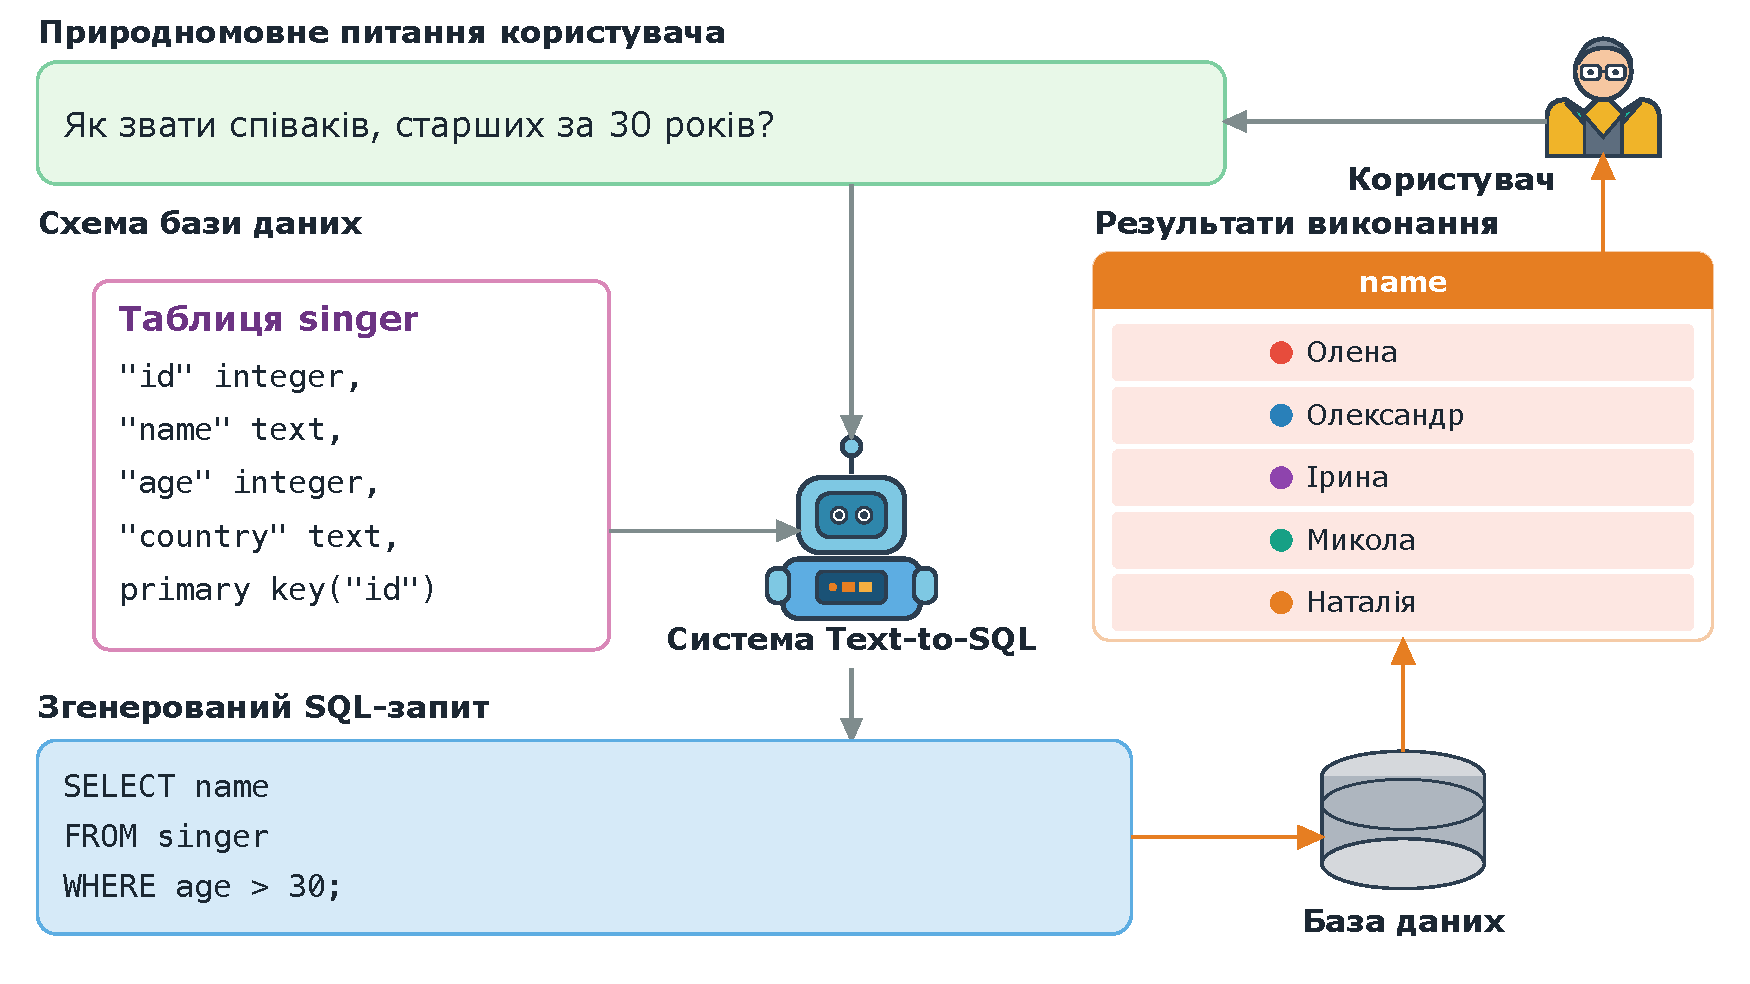
\includegraphics[width=\textwidth]{figures/skhema_text2sql_singer.pdf}
  \caption{Загальна схема природномовного доступу до бази даних із використанням систем Text-to-SQL}
  \label{fig:text2sql-overview}
\end{figure}

Семантична правильність запиту визначається його відповідністю змісту питання в контексті заданої бази. Різні за структурою SQL-запити можуть бути семантично еквівалентними. Водночас збіг результатів на одному стані \(D\) не доводить їхньої еквівалентності на інших станах. Наприклад, заміна \texttt{age > 30} на \texttt{age >= 30} у наведеному запиті змінює зміст умови. Проте обидва запити дадуть однакову відповідь, якщо в таблиці немає співаків віком рівно 30 років. Отже, слід розрізняти структурний збіг SQL, збіг результатів виконання та відповідність запиту питанню~\cite{shi2025survey}.

У наборах даних питанню \(q\) відповідає еталонний SQL-запит \(y^*\). Пару \((q,y^*)\) використовують для навчання та оцінювання систем. При цьому статус еталонного не гарантує правильності запиту.

Основні труднощі Text-to-SQL пов’язані з неоднозначністю природної мови, зіставленням понять питання з таблицями та колонками бази даних і визначенням потрібних SQL-операцій. Складні питання можуть вимагати з’єднання таблиць, агрегування та вкладених запитів. Окремою проблемою є узагальнення на нові схеми й предметні області, не представлені в навчальних даних.

% Авторегресивну факторизацію p_theta(y|x), параметри моделі та
% функцію втрат вводимо в 1.3 при викладі методів навчання.

\subsection{Еволюція підходів до Text-to-SQL}
\label{subsec:text2sql-evolution}

З погляду розвитку мовних моделей підходи до Text-to-SQL умовно поділяють на методи на основі правил, нейронні моделі, попередньо навчені мовні моделі (PLM) та великі мовні моделі (LLM)~\cite{liu2025survey}. Межі між цими групами не є чіткими, оскільки нові системи продовжують використовувати структурні обмеження й інші компоненти попередніх підходів. Водночас великі мовні моделі є масштабованим різновидом попередньо навчених моделей. Узагальнення розвитку підходів наведено на рис.~\ref{fig:text2sql-evolution}.

\begin{figure}[htbp]
  \centering
  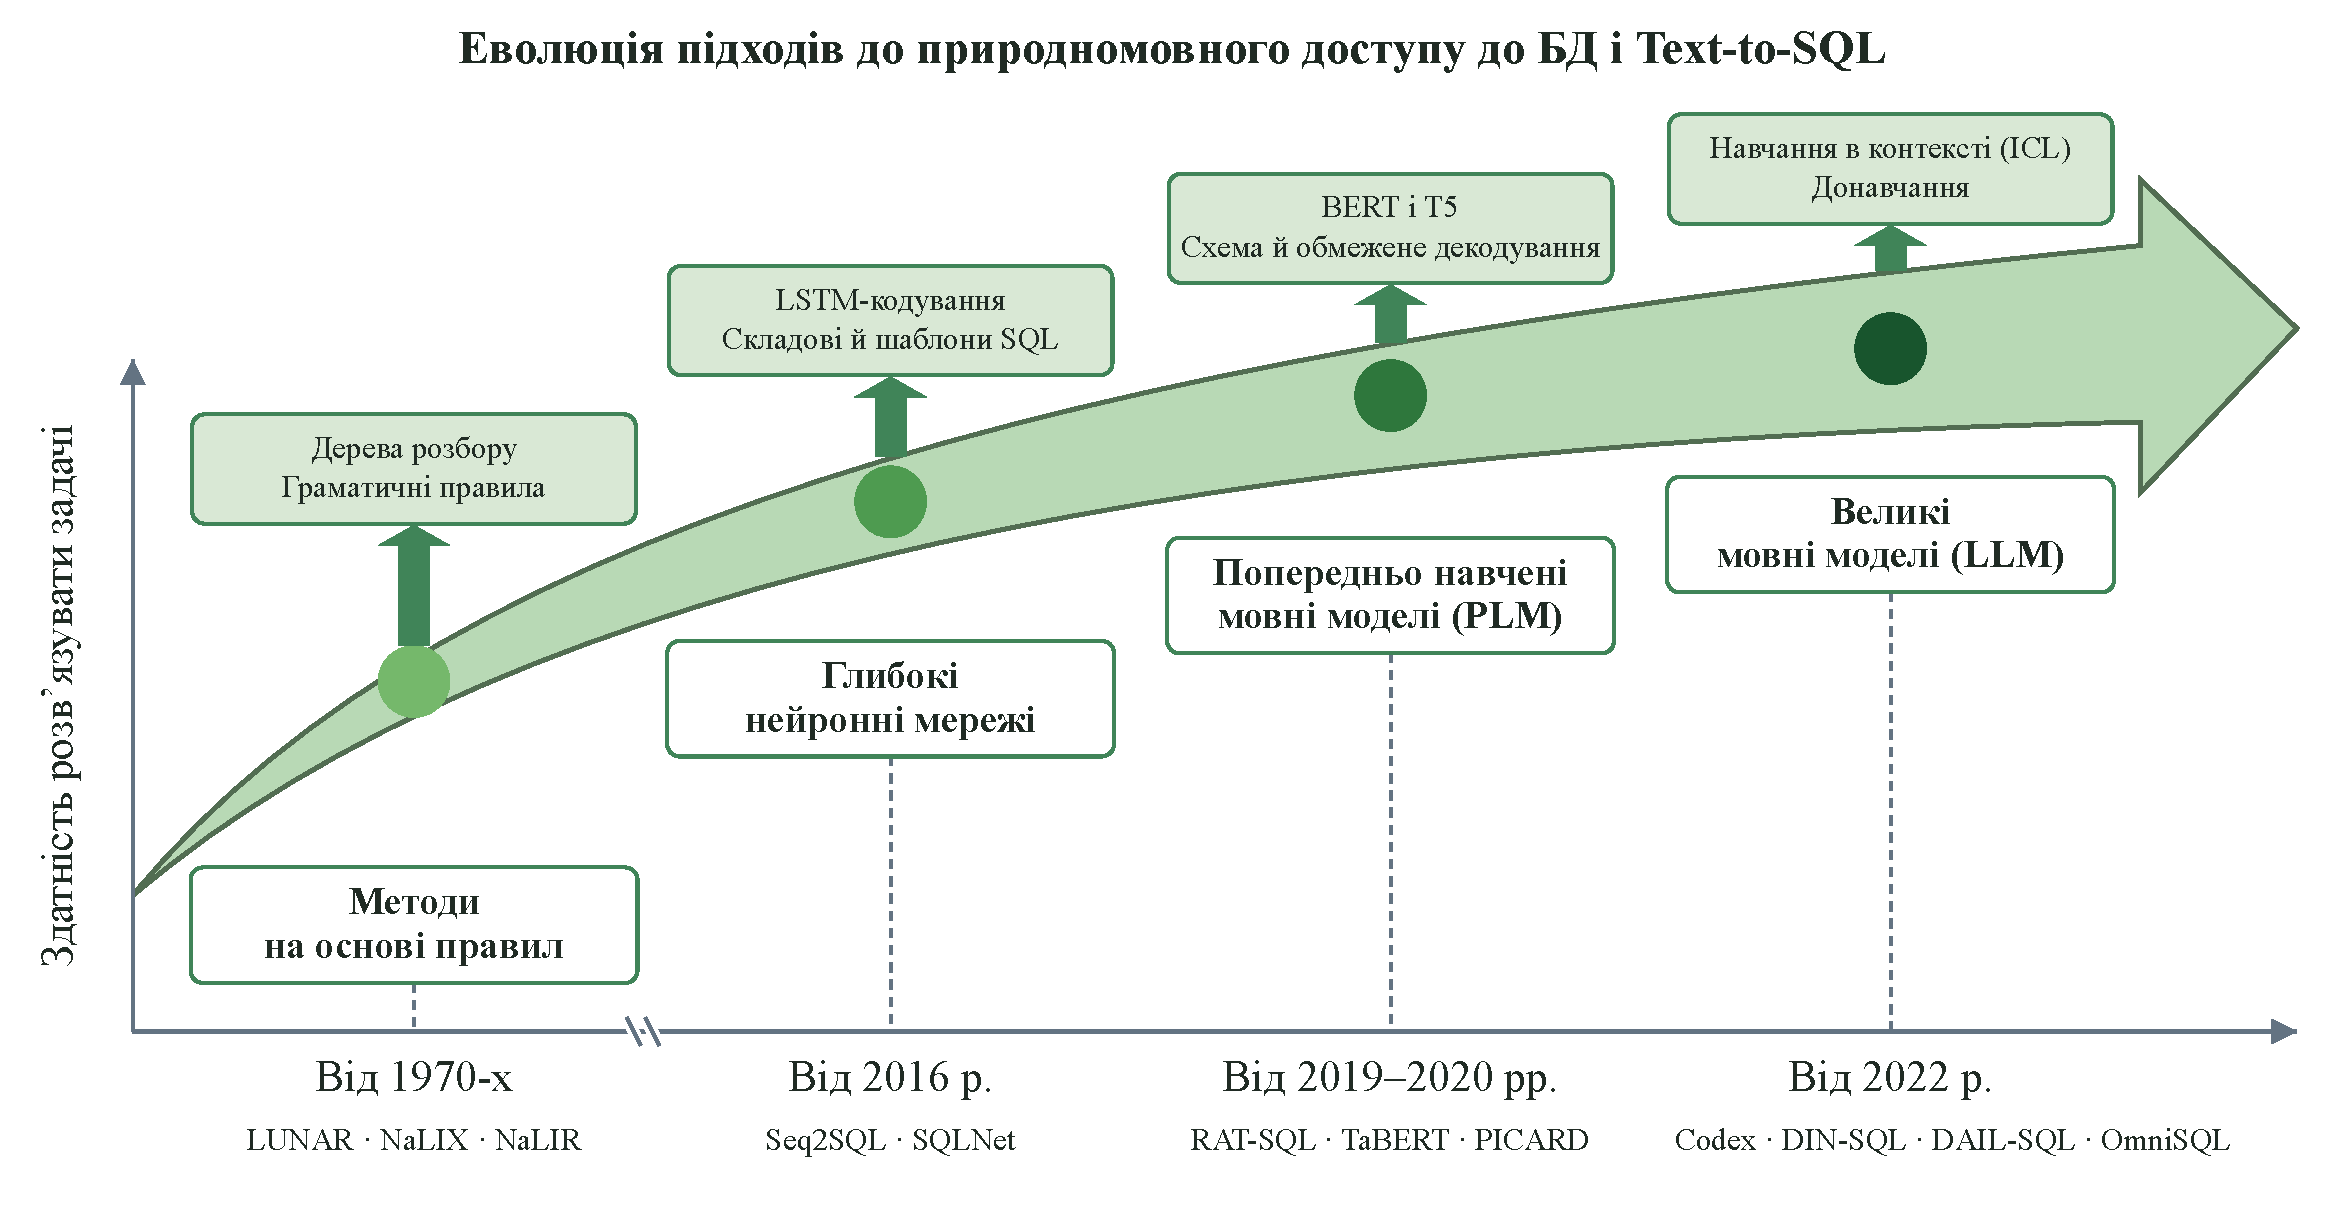
\includegraphics[width=\textwidth]{figures/evoliutsiia_text2sql.pdf}
  \caption{Еволюція підходів до природномовного доступу до баз даних і Text-to-SQL}
  \label{fig:text2sql-evolution}
\end{figure}

\textbf{Методи на основі правил і шаблонів.}
Типовий процес у системах на основі правил передбачав лексичний і синтаксичний аналіз питання. Синтаксичну структуру питання часто подавали як дерево синтаксичного розбору. Семантичні правила зіставляли елементи цього дерева з таблицями, колонками, значеннями та операціями над даними. За результатами зіставлення система формувала запит за визначеними правилами й шаблонами. Конкретний формат залежав від системи. LUNAR будувала процедуру отримання відповіді~\cite{woods1972lunar}, NaLIX~--- XQuery до XML-даних~\cite{li2005nalix}, а NaLIR~--- SQL-запит до реляційної бази~\cite{li2014nalir}.

Оскільки правила та відповідності задавали вручну, підтримка нових формулювань, елементів схеми й конструкцій запиту потребувала змін у системі. Це ускладнювало її супровід і перенесення на інші предметні області.

\textbf{Глибокі нейронні мережі.}
Із середини 2010-х років для семантичного парсингу почали застосовувати архітектури «кодувальник–декодувальник» на основі рекурентних нейронних мереж, зокрема LSTM. Dong і Lapata застосували LSTM із механізмом уваги для породження логічних форм, хоча їхня робота не була безпосередньо системою Text-to-SQL~\cite{dong2016logical}. На відміну від систем на основі правил, такі моделі навчали встановлювати відповідності між природномовним питанням і формальним запитом на основі навчальних прикладів. У Text-to-SQL такий приклад пов’язував питання і схему бази даних з еталонним SQL-запитом. Seq2SQL~\cite{zhong2017seq2sql} обирала агрегатну функцію й колонку для \texttt{SELECT}, а потім генерувала умови \texttt{WHERE}. Оскільки однакові умови можна записати в різному порядку, генератор \texttt{WHERE} навчали з підкріпленням і оцінювали не дослівний збіг з еталоном, а результат виконання запиту. SQLNet~\cite{xu2017sqlnet}, у свою чергу, розв’язувала ту саму проблему без навчання з підкріпленням. Вона заповнювала складові фіксованого шаблону SQL і передбачала колонки умов як невпорядковану множину із механізмом уваги до колонок.

\textbf{Попередньо навчені мовні моделі.}
Наприкінці 2010-х років у Text-to-SQL почали використовувати попередньо навчені трансформерні моделі. Ключовою відмінністю від попереднього етапу стало попереднє навчання моделі на великих текстових корпусах із подальшою адаптацією до Text-to-SQL. Під час адаптації модель донавчали на прикладах, що пов’язували питання і схему бази даних з еталонним SQL-запитом. RAT-SQL кодувала зв’язки між елементами схеми та відповідності між словами питання й елементами схеми за допомогою механізму самоуваги з урахуванням відношень. У варіанті RAT-SQL + BERT початкові представлення слів питання й назв елементів схеми отримували за допомогою BERT~\cite{wang2020ratsql}. TaBERT створили шляхом продовження попереднього навчання BERT на таблицях і пов’язаних із ними текстах. Потім TaBERT використовували як кодувальник у семантичному парсері та донавчали разом із ним на прикладах Text-to-SQL~\cite{yin2020tabert}. У PICARD під час декодування донавченої T5 інкрементальний синтаксичний аналіз відхиляв токени, які не могли бути допустимим продовженням SQL-запиту~\cite{scholak2021picard}.

\textbf{Великі мовні моделі.}
Перехід до великих мовних моделей був пов’язаний із масштабуванням попередньо навчених моделей за кількістю параметрів, обсягом навчальних даних і обчислювальними витратами. Довше контекстне вікно давало змогу одночасно подавати моделі інструкцію, опис схеми бази даних та, за потреби, приклади «питання~--- SQL». У 2022~році Rajkumar та ін. показали можливість використання Codex для генерації SQL у такій постановці без спеціалізованого донавчання~\cite{rajkumar2022evaluating}. DIN-SQL розкладає задачу на зв’язування зі схемою, декомпозицію, генерацію SQL і самокорекцію~\cite{pourreza2023dinsql}. DAIL-SQL досліджує добір і подання прикладів для навчання в контексті~\cite{gao2024benchmark}. Водночас донавчання зберегло своє значення. Великі мовні моделі донавчають повністю або оновлюють лише невелику частину параметрів, наприклад низькорангові адаптери LoRA~\cite{liu2025survey,hu2022lora}. Зокрема, моделі OmniSQL донавчено на синтетичному наборі SynSQL-2.5M разом із навчальними частинами Spider і BIRD, а цільова відповідь містить покрокове пояснення та фінальний SQL-запит~\cite{li2025omnisql}.

% Нижче збережено попередній чорновик. Перенесення метрик до 1.2.3
% та написання 1.1.3 виконуються на наступних етапах.
\subsection{Метрики exact match і execution accuracy}

Еталони систем Text-to-SQL використовують метрики, які охоплюють і правильність SQL-запиту, і його ефективність. Цими метриками перевіряють, що система дає точний SQL і що запит виконується ефективно на справжніх базах. Метрики поділяються на дві групи: зіставлення вмісту і оцінювання за результатом виконання~\cite{mohammadjafari2024review}. Рисунок~\ref{fig:metrics} показує чотири метрики цієї класифікації на одному питанні і одному еталонному запиті.

Нехай \(N\) — кількість прикладів, \(Y_n\) — еталонний запит \(n\)-го прикладу, а \(\hat{Y}_n\) — згенерований. \(V_n\) і \(\hat{V}_n\) — результати виконання цих запитів на тій самій базі. Індикатор \(\mathbf{1}(\cdot)\) дорівнює 1, якщо умова в дужках виконана, і 0 інакше.

\begin{figure}[htbp]
  \centering
  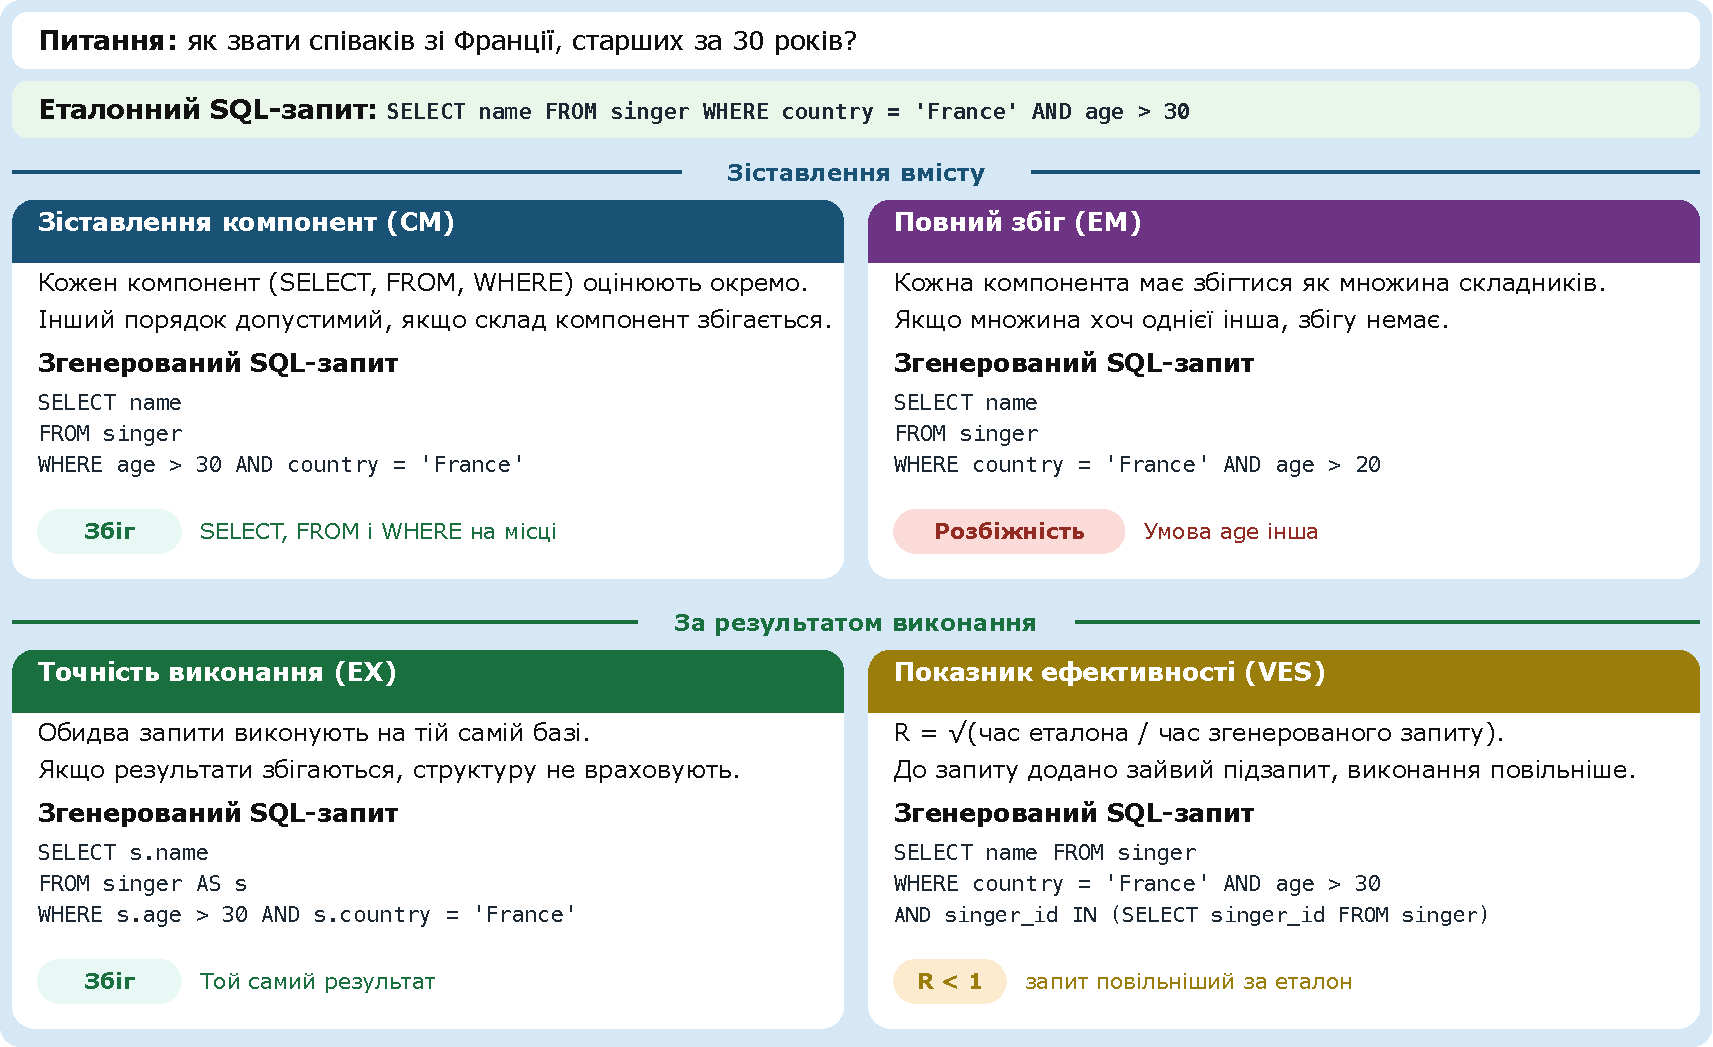
\includegraphics[width=\textwidth]{figures/metryky.pdf}
  \caption{Чотири метрики оцінювання за оглядом Mohammadjafari et al. Зіставлення компонент і повний збіг дивляться на структуру запиту. Точність виконання і показник ефективності дивляться на результат і на час.}
  \label{fig:metrics}
\end{figure}

Зіставлення вмісту дивиться, наскільки структура згенерованого запиту збігається зі структурою еталонного. Таке оцінювання потрібне, щоб перевірити, чи модель дотримується правильного синтаксису і структури SQL, навіть якщо запит не завжди є найекономнішим~\cite{mohammadjafari2024review}.

Зіставлення компонент (component matching, CM) оцінює кожен компонент запиту окремо, зокрема \texttt{SELECT}, \texttt{FROM} і \texttt{WHERE}~\cite{mohammadjafari2024review,yu2018spider}. Нехай \(A(Y_n^{C})\) — множина складників компоненти \(C\) еталонного запиту, а \(A(\hat{Y}_n^{C})\) — множина складників тієї самої компоненти згенерованого. Порядок складників до множини не входить:
\begin{equation}
\label{eq:cm}
CM^{C}
= \frac{1}{N} \sum_{n=1}^{N}
\mathbf{1}\bigl(A(Y_n^{C}) = A(\hat{Y}_n^{C})\bigr).
\end{equation}
На рисунку для \texttt{WHERE} складники ті самі: \texttt{country = 'France'} і \texttt{age > 30}, тож індикатор дорівнює 1. Для \texttt{ORDER BY} і \texttt{HAVING} порядок складників зберігають; рисунок цих компонент не показує.

Повний збіг (exact matching, EM) вимагає того самого збігу від кожної компоненти. Нехай \(\mathcal{C}\) — компоненти запиту. Тоді
\begin{equation}
\label{eq:em}
EM
= \frac{1}{N} \sum_{n=1}^{N}
\mathbf{1}\Bigl(\bigwedge_{C \in \mathcal{C}}
\bigl(A(Y_n^{C}) = A(\hat{Y}_n^{C})\bigr)\Bigr).
\end{equation}
Індикатор дорівнює 1 лише тоді, коли рівність множин виконана для кожної \(C \in \mathcal{C}\). Переставлення умов усередині однієї компоненти повного збігу не ламає~\cite{yu2018spider}. Зв'язка до множини \texttt{WHERE} не входить: це окрема компонента, \(\{\texttt{AND}\}\) і \(\{\texttt{OR}\}\) не рівні, тож заміна однієї на іншу повного збігу не дає. Підзапит усередині \texttt{WHERE} є одним складником цієї множини і не дописується до зовнішніх \texttt{SELECT} і \texttt{FROM}. На рисунку в згенерованому запиті стоїть \texttt{age > 20} замість \texttt{age > 30}, тож множина \texttt{WHERE} інша і повного збігу немає. Запит, правильний за результатом, усе одно не зараховують, якщо множина складників хоч однієї компоненти інша~\cite{mohammadjafari2024review}.

Оцінювання за результатом виконання дивиться на фактичну роботу згенерованого запиту, коли його виконують на базі. Ці метрики перевіряють, що запит дотримується правильної структури, повертає правильний результат і виконується ефективно в реальних умовах~\cite{mohammadjafari2024review}.

Точність виконання (execution accuracy, EX) перевіряє, чи згенерований запит, виконаний на базі, повертає той самий результат, що й еталонний~\cite{mohammadjafari2024review,yu2018spider}:
\begin{equation}
\label{eq:ex}
EX
= \frac{1}{N} \sum_{n=1}^{N}
\mathbf{1}(V_n = \hat{V}_n).
\end{equation}
Метрика дивиться на правильність результату незалежно від структури запиту. Для прикладу зі співаками інший текст із тим самим результатом зберігає точність виконання. Збіг порожніх результатів можливий і тоді, коли обидва запити не відповідають питанню; метрика залежить від вмісту бази~\cite{finegandollak2018evaluation,shi2025survey}.

Показник ефективності (valid efficiency score, VES) вимірює обчислювальну ефективність згенерованого запиту порівняно з еталонним. Запит може повернути правильний результат і водночас бути неефективним, бо потребує зайвих обчислень. Метрика карає додаткову складність, зокрема зайвий підзапит або зайве з'єднання, навіть за збігу результатів~\cite{li2023bird,mohammadjafari2024review}. На \(N\) прикладах VES оцінює і правильність, і ефективність кожного згенерованого запиту:
\begin{equation}
\label{eq:ves}
\mathrm{VES}
= \frac{1}{N} \sum_{n=1}^{N}
\mathbf{1}(V_n = \hat{V}_n) \cdot R(Y_n, \hat{Y}_n),
\end{equation}
де відносна ефективність
\begin{equation}
\label{eq:ves-r}
R(Y_n, \hat{Y}_n) = \sqrt{\frac{E(Y_n)}{E(\hat{Y}_n)}}
\end{equation}
є коренем із відношення часу виконання еталонного запиту до часу згенерованого. Підсумковий VES є середнім цих величин за всіма \(N\) прикладами. Оцінка 1 означає водночас точність і оптимальну ефективність~\cite{mohammadjafari2024review}. На великих базах BIRD головними метриками є EX і VES, бо одну відповідь записують різними коректними запитами~\cite{li2023bird}.

Порівнянними числа повного збігу й точності виконання різних систем є тоді, коли вони пораховані на тих самих золотих парах і на тому самому авторському розбитті. Це розбиття задають набори, розглянуті далі.

\section{Еталонні та навчальні набори даних}

Еталонний набір і навчальний виконують різні ролі. Еталон (WikiSQL, Spider, BIRD) має авторське розбиття і золоті пари, тож exact match і execution accuracy різних систем ставлять поряд. Навчальним є train-частина Spider чи BIRD або синтетичний корпус, на якому модель донавчають. Автоматичний поділ рядків набору, викладеного на Hugging Face, дає тестову частку, але не еталон: офіційні train і dev Spider розведені за базами, і статті звітують саме на цьому розбитті~\cite{yu2018spider,finegandollak2018evaluation}. Випадкова частка рядків, особливо коли одна схема потрапляє в обидві частини, дає непорівнянне число.

\subsection{WikiSQL і Spider}

WikiSQL є одним із перших великих наборів Text-to-SQL: 80\,654 пари «питання~--- SQL» на 24\,241 таблиці Вікіпедії~\cite{zhong2017seq2sql}. Запит стосується однієї таблиці. З’єднання, вкладені підзапити і складна агрегація в постановку не входять. Оцінювання ведуть за збігом логічної форми і за точністю виконання.

Spider знімає це обмеження і фіксує міждоменне оцінювання~\cite{yu2018spider}. У наборі 10\,181 питання і 5\,693 унікальні SQL-запити на 200 базах у 138 доменах. Схеми містять кілька таблиць і зовнішні ключі. Запити покривають вкладеність, операції над множинами і групування з агрегацією. Питання писали студенти, які володіють SQL; пари проходили окремий перегляд SQL, перегляд питання і фінальний перегляд. Train і dev розведені за базами: схеми dev у навчанні відсутні. Через це Spider лишається опорним еталоном міждоменного Text-to-SQL~\cite{shi2025survey,gao2024benchmark}.

Поділ за питаннями, а не за базами, завищує оцінку узагальнення на нові запити~\cite{finegandollak2018evaluation}. Тому dev Spider, узятий з офіційного розбиття, і тестова частка, нарізана з таблиці Hugging Face за рядками, є різними об’єктами вимірювання.

\subsection{BIRD}

BIRD переносить ту саму міждоменну постановку на великі бази з брудними значеннями~\cite{li2023bird}. У наборі 12\,751 пара на 95 базах у 37 професійних доменах; сумарний обсяг баз близько 33~ГБ. Питання і SQL анотують різні люди, SQL проходить подвійне сліпе анотування і експертний перегляд.

Окремо від Spider BIRD стоїть через поле \texttt{evidence}. Це коротка підказка анотації: яке значення якої колонки відповідає словам питання. Питання часто не розв’язується з самих імен таблиць і колонок, бо в тексті є зовнішнє знання і реалістичні значення. Поле \texttt{evidence} є частиною пункту набору. Діалоговий контекст попередніх реплік, як у SParC~\cite{yu2019sparc} і CoSQL~\cite{yu2019cosql}, до цього поля не входить: BIRD лишається набором окремих питань.

Друга відмінність~--- обсяг баз. Поряд зі збігом результату дивляться ефективність виконання, тож головні метрики BIRD~--- EX і VES~\cite{li2023bird}. Spider для подальшого експерименту адаптації лишається набором із компактними базами і розбиттям за схемами; BIRD у цьому розділі потрібен як еталон, де золота пара несе ще й підказку \texttt{evidence}.

\subsection{Синтетичні корпуси Gretel і OmniSQL}

Ручна анотація Spider і BIRD обмежена в обсязі, тому для донавчання збирають синтетичні корпуси. Gretel-Synth містить понад 100\,000 прикладів у ділових доменах і поширюється як набір Hugging Face~\cite{gretel2024synth}. OmniSQL доводить масштаб далі: понад 2,5~млн екземплярів на більш ніж 16\,000 синтетичних базах, із ланцюжком міркувань біля запиту~\cite{li2025omnisql}.

Такий корпус є навчальним матеріалом. Авторського розбиття, на якому різні системи звітують exact match і execution accuracy, у нього немає. Зростання обсягу саме по собі якість пар не гарантує. У дослідженні Arctic-Text2SQL додавання нижчої за якістю синтетики, зокрема Gretel-Synth, знижувало точність, попри більший train~\cite{yao2025arctic}. Для донавчання істотним є вміст пар, а не лише їхня кількість.

\section{Методи адаптації великих мовних моделей до задачі Text-to-SQL}

Мовну модель, уже навчену на широкому корпусі, підводять до Text-to-SQL двома режимами: без оновлення параметрів і з їхнім оновленням~\cite{shi2025survey,mohammadjafari2024review,gao2024benchmark}. Далі розібрано повне донавчання, навчання з кількох прикладів і параметрично ефективну адаптацію, на якій стоїть залежність якості моделі від якості навчальних пар.

\subsection{Повне донавчання і навчання з кількох прикладів}

Повне донавчання оновлює всі параметри моделі на парах «питання і схема~--- SQL». Функція втрат~--- перехресна ентропія наступного токена, порахована на токенах золотого SQL; токени питання і схеми в втрату не входять. Режим потребує великого train і пам’яті на всі ваги та стани оптимізатора. Для моделі з мільярдами параметрів повне оновлення є дорогим навіть тоді, коли змінюється лише вузька задача.

Навчання з кількох прикладів (few-shot, in-context learning) параметрів не змінює. У контекст кладуть схему, саме питання і кілька золотих пар як зразок~\cite{gao2024benchmark,shi2025survey}. Застосування швидке, окремий цикл навчання відсутній. Обмеженням є довжина контексту: повна схема великої бази і кілька довгих запитів можуть у неї не ввійти. Ваги лишаються тими, що були до прикладу, тож дефект навчального корпусу в параметри моделі цим режимом не записується. Він впливає лише на ті пари, які потрапили в конкретний контекст.

Для задачі, де треба виміряти вплив корпусу на саму модель, потрібен режим, у якому навчається невелика добавка до фіксованих ваг. Його задають LoRA і QLoRA.

\subsection{LoRA і QLoRA}

LoRA лишає матрицю ваг попередньо навченої моделі фіксованою і навчає добавку низького рангу~\cite{hu2022lora}. Для лінійної проєкції з входом \(x\) вихід має вигляд
\begin{equation}
\label{eq:lora}
h = W_0 x + \frac{\alpha}{r} B A x,
\end{equation}
де \(W_0\) не оновлюється, \(A\) і \(B\)~--- матриці рангу \(r\), значно меншого за розміри \(W_0\), а \(\alpha / r\)~--- масштабний коефіцієнт. \(A\) ініціалізують випадково, \(B\)~--- нулем, тож на початку навчання добавка нульова і вихід збігається з виходом фіксованої проєкції. Градієнт іде в \(A\) і \(B\). Після навчання добавку можна злити з \(W_0\) і отримати одну матрицю без додаткової затримки на виведенні~\cite{hu2022lora}.

\begin{figure}[htbp]
  \centering
  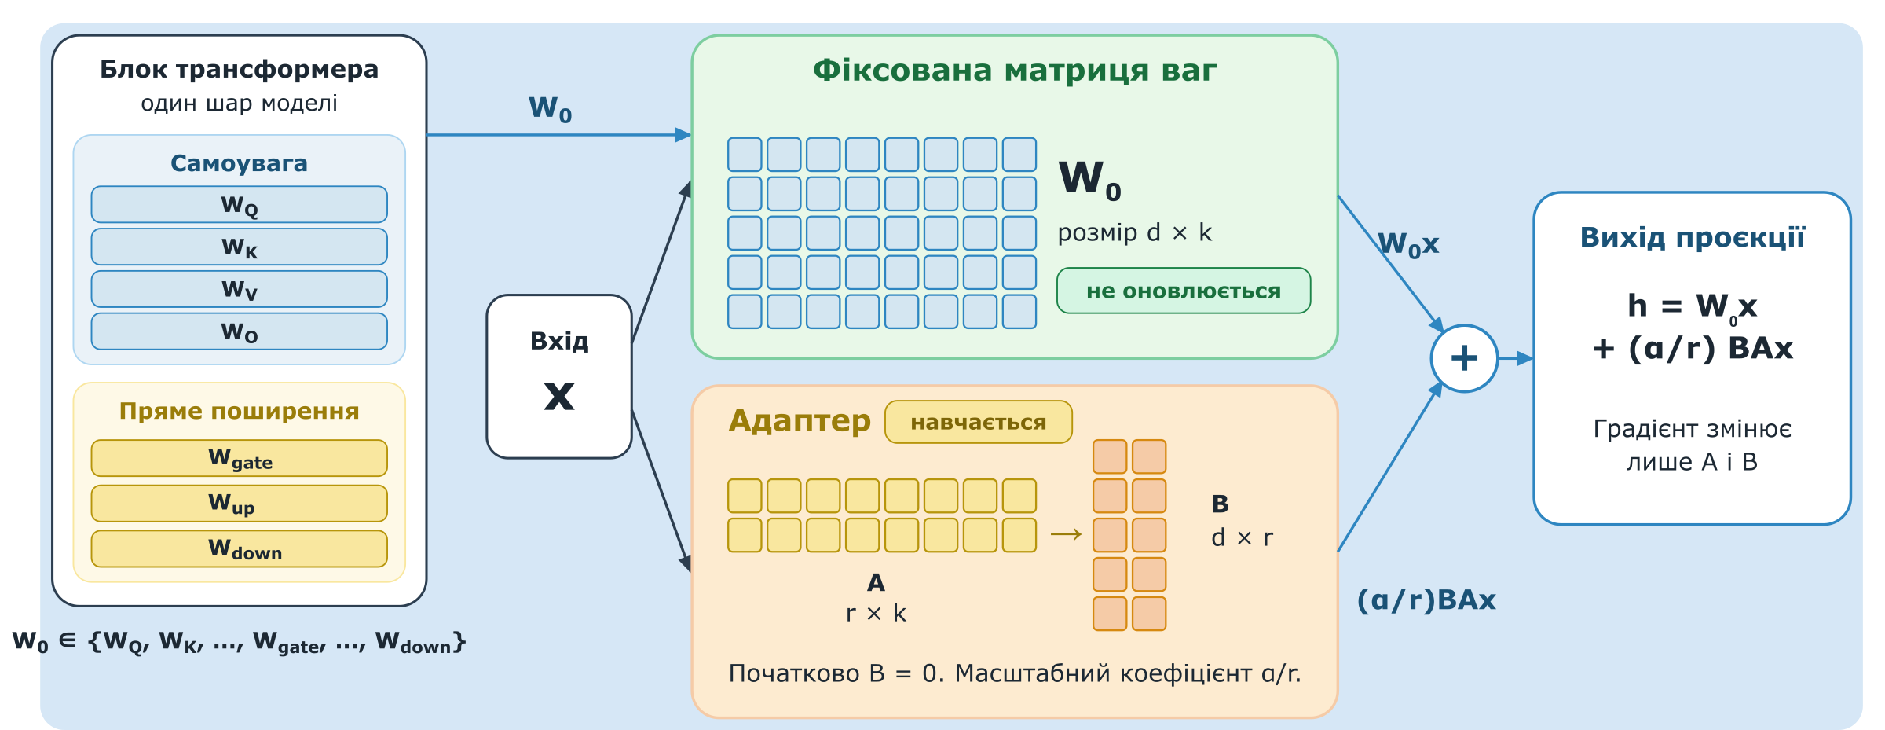
\includegraphics[width=\textwidth]{figures/lora_shar.pdf}
  \caption{Низькорангова добавка до лінійної проєкції. \(W_0\) фіксована; навчаються \(A\) і \(B\). Початково \(B = 0\).}
  \label{fig:lora}
\end{figure}

Рисунок~\ref{fig:lora} показує одну таку проєкцію. У блоці трансформера та сама добавка може стояти на проєкціях уваги \(W_Q\), \(W_K\), \(W_V\), \(W_O\) і на трьох проєкціях блока прямого поширення \(W_{\mathrm{gate}}\), \(W_{\mathrm{up}}\), \(W_{\mathrm{down}}\). Hu et al.\ вводять метод на проєкціях уваги~\cite{hu2022lora}; для моделей зі SwiGLU той самий розклад застосовують і до блока прямого поширення. Саме цей набір проєкцій використовує подальший експеримент адаптації.

QLoRA зберігає той самий цикл і ту саму формулу~\eqref{eq:lora}~\cite{dettmers2023qlora}. Відмінність у тому, як зберігається \(W_0\): її квантують до 4-бітного NormalFloat (NF4), константи квантування квантують ще раз (подвійне квантування), а для множення матрицю деквантують у 16-бітний обчислювальний тип. Градієнт ваг рахують лише для адаптера. Огляд родини LoRA ставить QLoRA серед методів, які зменшують пам’ять~\cite{mao2025lorasurvey}. На вимірюваннях Dettmers et al.\ якість QLoRA тримається на рівні 16-бітного донавчання; виграш полягає в пам’яті, потрібній для адаптації, а не в іншій функції втрат~\cite{dettmers2023qlora}. Окремої схеми обчислення для QLoRA цей розділ не вводить: її задає рисунок~\ref{fig:lora} разом із квантованим зберіганням \(W_0\).

\subsection{Залежність якості адаптації від якості навчальних даних}

У режимі~\eqref{eq:lora} оновлюється невелика добавка, а сигнал для неї дають золоті SQL. Дефект пари входить у втрату нарівні з коректною парою: модель підганяє адаптер до того тексту запиту, який стоїть у train. Тому якість навчальних пар є змінною адаптації, а не лише властивістю еталонної таблиці.

Чутливість Text-to-SQL до вмісту даних зафіксовано й поза донавчанням. Dr.Spider задає 17 типів збурень бази, питання і SQL. На найстійкішій із перевірених моделей відносне падіння усередненої точності виконання становить 14,0~\%, а на збуренні еквівалентного вмісту бази~--- 50,7~\%~\cite{chang2023drspider}. Це оцінювання готових систем, і воно показує, що невелика зміна даних змінює виміряну якість.

Для самого навчання той самий висновок дають два незалежні спостереження. QLoRA на невеликому інструкційному наборі високої якості досягає рівня сильніших режимів донавчання~\cite{dettmers2023qlora}. У Text-to-SQL додавання великого, але слабшого синтетичного корпусу здатне погіршити точність~\cite{yao2025arctic}. Обсяг train і придатність пар до навчання розходяться.

Окремо показано, що помилки золотих пар змінюють порівняння систем навіть без донавчання. Jin et al.\ оцінюють частку помилкових анотацій у 52,8~\% на BIRD Mini-Dev і 62,8~\% на Spider~2.0-Snow. Після виправлення підмножини зі 100 пунктів BIRD Dev вони наново міряють 16 відкритих агентів: відносна зміна якості лежить у межах від \(-7\) до \(+31\)~\%, зсув місця в рейтингу~--- від \(-9\) до \(+9\), а кореляція Спірмена між початковим і виправленим рейтингами падає з 0,85 до 0,32~\cite{jin2026annotation}. Автори переоцінюють готові агенти і ваги моделей не оновлюють. Питання про те, як виправлення train змінює QLoRA-адаптацію, цим виміром не закрите. Воно потребує засобів, які спочатку відокремлюють різні дефекти пар.

\section{Контроль якості анотацій і наявні засоби аудиту}

Дефект золотої пари буває різним за природою. Запит може бути синтаксично прийнятним і водночас містити відомий антипатерн SQL. Він може виконуватися і при цьому не відповідати питанню. Схема або вміст бази можуть бути неузгоджені самі по собі, ще до тексту питання. Далі засоби розведено за цими трьома предметами перевірки.

\subsection{Виявлення антипатернів SQL}

Каталог повторюваних хиб SQL і проєктування баз зібрано в Karwin~\cite{karwin2010sqlantipatterns}: запит є припустимим для рушія і водночас ненадійний за сенсом або за поведінкою на крайових даних. SQLCheck переносить частину цього каталогу в автоматичні правила і діагностує антипатерн окремого запиту~\cite{dintyala2020sqlcheck}.

Для аудиту наборів Text-to-SQL цього замало з двох причин. SQLCheck працює з одним запитом, а не з корпусом золотих пар Spider, BIRD чи синтетичного набору, і не веде діалект, у якому ці пари написано. Покриття правил також вужче за простір, істотний для таких корпусів: поза ним лишаються небезпечні запити зміни даних, порядкозалежна пагінація і шаблони підзапитів, чутливі до \texttt{NULL}~\cite{dintyala2020sqlcheck,karwin2010sqlantipatterns}.

Отже, відкритим лишається діалектне виявлення антипатернів у золотих запитах Spider, BIRD і синтетичних корпусів, разом із класами, які SQLCheck не бере. Цей предмет належить розділу~2.

\subsection{Перевірка семантичної відповідності питання і SQL}

Профілювання корпусу описує набір у цілому і не вирішує, чи узгоджена конкретна золота пара. Mitsopoulou і Koutrika зіставляють набори за структурою SQL, властивостями схеми і лексикою питань і розкладають помилки моделі на структурні, операторні й змінні~\cite{mitsopoulou2025analysis}. Процедура придатна для порівняння корпусів і розбору помилок систем. Вердикту про окрему анотацію вона не виносить.

Перевірку окремих пар ведуть кількома лініями, і в автоматичній частині вони спираються на мовну модель. NL2SQL-BUGs дає 2\,018 експертно розмічених перекладів, із них 999 із семантичними помилками, і дворівневу таксономію таких помилок. Окремо автори просіюють Spider і BIRD моделлю GPT-4o і підтверджують знайдені помилки вручну; виконуваного конвеєра на весь корпус у випуску немає~\cite{liu2025nl2sqlbugs}. Jin et al.\ будують агента, який кілька кроків працює з базою і складає діагностичний звіт; остаточне рішення лишається за експертом, після чого анотацію виправляють~\cite{jin2026annotation}. SQLDriller породжує альтернативні SQL, шукає бази-контрприклади і порівнює результат виконання з тим, який модель передбачає за питанням; за розбіжністю пару позначають і виправляють, а виправлений train Spider і BIRD використовують для донавчання~\cite{yang2025sqldriller}. Спільним для цих ліній є те, що семантичне рішення або його частина залежить від моделі, від людини або від обох.

Детерміновані правила в розглянутих роботах розв’язують сусідню задачу. BLEC зіставляє ключові слова згенерованого тексту з семантичним розбором і зводить три типи правил~--- заперечення, оператори, словник набору~--- до бінарної мітки корпусу~\cite{shu2021blec}. Нерозв’язного випадку, коли правилу бракує доказу, метод не має. PV-SQL витягає з питання і необов’язкового \texttt{evidence} десять типів обмежень і перевіряє, чи містить згенерований SQL потрібні конструкції~\cite{tian2026pvsql}. Перевірка вбудована в цикл агента і скеровує виправлення під час виведення. Об’єктом є згенерований запит, а не збережена золота пара. Розбіжність автори відносять до витягнутого обмеження. Обмеження поза набором шаблонів опускають, окремого нерозв’язного статусу вони не отримують.

Отже, відкритою лишається детермінована перевірка збережених пар «питання~--- золотий SQL» на масштабі корпусу: кожна знахідка має спиратися на явний доказ із питання або зі запиту, брак доказу має давати окремий нерозв’язний випадок, а повторюваність шаблону в корпусі не є доказом його правильності. Цей предмет належить розділу~3. Комітет мовних моделей як ширша семантична перевірка розглянуто в наступному пункті; його виміри до цього розділу не входять.

\subsection{Перевірка схеми, даних і оцінювання комітетом мовних моделей}

Схема і вміст бази є окремим предметом, бо пара може бути внутрішньо узгодженою, а база, на якій її виконують,~--- ні. Реляційне профілювання виявляє залежності включення, унікальні комбінації колонок і кандидати у зовнішні ключі~\cite{abedjan2015profiling}. Для наборів на SQLite істотною є поведінка зовнішнього ключа за вимкненого примусового контролю і за семантики \texttt{NULL}: порушення посилань тоді не зупиняє запис рядка~\cite{memari2015sql}. Саме так зібрано бази Spider~1.0. SchemaCrawler додає огляд схеми і перевірки на зразок статичного аналізу~\cite{schemacrawler}. Ці засоби дивляться на схему і на відношення як на самостійні артефакти. Знахідка не прив’язана до пункту «питання~--- SQL».

Виконання запиту на базі є третьою, вже динамічною перевіркою: запит може розібратися і при цьому впасти на даних або повернути результат, який не випливає з питання. Синтаксична прийнятність, антипатерн, семантика пари і виконуваність на конкретній базі дають різні списки дефектів. Злиття цих списків в одну позначку «пара погана» стирає, який саме дефект виправлено.

Там, де правило не має доказу, семантику оцінюють комітетом мовних моделей. Сильний суддя наближає людські переваги і водночас має зміщення позиції, багатослівності, самопідсилення і слабку ділянку міркувань~\cite{zheng2023judgingllm}. Комітет і обмін аргументами між суддями зменшують залежність від однієї моделі і виводять розбіжність назовні~\cite{chan2024chateval}. Для аудиту Text-to-SQL звідси випливає режим користування, а не заміна еталона: контрольована підказка, кілька моделей, рішення більшістю і подальше калібрування людиною. Вердикт комітету є сигналом, який треба підтвердити, перш ніж правити золоту пару.

Таблиця~\ref{tab:audit-means} зводить засоби цього підрозділу і двох попередніх за предметом перевірки і за тим, чого бракує для аудиту корпусу золотих пар.

\begin{table}[htbp]
  \caption{Засоби контролю якості анотацій Text-to-SQL}
  \label{tab:audit-means}
  \small
  \renewcommand{\arraystretch}{1.15}
  \begin{tabularx}{\textwidth}{@{}>{\raggedright\arraybackslash}p{3.3cm} >{\raggedright\arraybackslash}X >{\raggedright\arraybackslash}X@{}}
    \toprule
    Засіб & Що перевіряє & Обмеження для аудиту корпусу \\
    \midrule
    Mitsopoulou, Koutrika~\cite{mitsopoulou2025analysis} &
    структуру SQL, схему, лексику питань &
    немає вердикту про окрему золоту пару \\
    SQLCheck~\cite{dintyala2020sqlcheck} &
    антипатерни одного запиту &
    не корпус і не діалект; частина класів поза правилами \\
    BLEC~\cite{shu2021blec} &
    ключові слова тексту проти розбору &
    бінарна мітка; нерозв’язного випадку немає \\
    PV-SQL~\cite{tian2026pvsql} &
    обмеження в згенерованому SQL &
    золоту анотацію не аудитує \\
    NL2SQL-BUGs~\cite{liu2025nl2sqlbugs} &
    семантичні помилки перекладу &
    немає конвеєра на весь корпус \\
    Jin et al.~\cite{jin2026annotation} &
    семантику анотації агентом &
    рішення моделі і людини; донавчання немає \\
    SQLDriller~\cite{yang2025sqldriller} &
    узгодженість за виконанням і виправлення &
    донавчання після ремонту без поділу груп правок \\
    Профілювання схеми~\cite{abedjan2015profiling,memari2015sql,schemacrawler} &
    ключі, залежності, цілісність &
    знахідка не прив’язана до пари питання~--- SQL \\
    \bottomrule
  \end{tabularx}
\end{table}

Jin et al.\ після виправлення наново міряють готових агентів і ваги не оновлюють~\cite{jin2026annotation}. SQLDriller уже донавчає модель на виправленому train~\cite{yang2025sqldriller}. В обох випадках виправлення злито: з результату не видно, який внесок дають окремо антипатерни, семантичні суперечності, підтверджені знахідки комітету і дефекти схеми та даних.

Отже, відкритим лишається багатовимірний аудит, у якому ці чотири джерела правок зберігають окремі списки, і вимірювання того, як кожне джерело змінює QLoRA-адаптацію на авторському розбитті Spider. Цей предмет належить розділу~4.

\section*{Висновки до розділу 1}

Огляд фіксує задачу як перехід від питання і схеми до SQL, а якість розв’язку~--- як повний збіг форми і як збіг результату виконання. Еталонні набори WikiSQL, Spider і BIRD дають золоті пари й авторське розбиття, на якому ці метрики порівнянні. BIRD додає поле \texttt{evidence} і ефективність виконання на великих базах. Gretel і OmniSQL є навчальними корпусами: масштаб у них великий, а лідербордної ролі немає. Адаптацію, у якій дефект пари здатний увійти в параметри, задає QLoRA: фіксована матриця зберігається квантованою, навчається низькорангова добавка.

Зіставлення засобів контролю залишає три прогалини.

Діалектного виявлення антипатернів у золотих запитах Spider, BIRD і синтетичних корпусів, із класами поза правилами SQLCheck, наявні засоби не дають. Цю прогалину закриває розділ~2.

Детермінованої перевірки збережених пар «питання~--- золотий SQL», із явним доказом і окремим нерозв’язним випадком, розглянуті методи не дають: або рішення залежить від моделі, або правило обслуговує генерацію і не аудитує золоту анотацію. Цю прогалину закриває розділ~3.

Вплив чотирьох окремих груп виправлень на QLoRA-адаптацію не виміряно. Виправлення анотацій або змінює рейтинг готових агентів без донавчання, або входить у донавчання вже злитим корпусом. Цю прогалину закриває розділ~4.

\bibliographystyle{unsrtnat}
\bibliography{rozdil_1}

\end{document}
